\documentclass[a4paper,10pt]{article}

\usepackage{exercices}
\usepackage{nicefrac}
\usepackage{multirow}
\usepackage{color}
\usepackage{listings,fancyvrb}

\usepackage{fullpage}%
\usepackage{multicol}
\usepackage{tikz}

%\usepackage[francais]{babel}%
\usepackage[T1]{fontenc}%

\usepackage{listings}%
\lstset{%
  basicstyle=\sffamily,%
  columns=fullflexible,%
  language=C++,%
  frame=lb,%
  frameround=fftf,%
}%

\newcommand{\code}[1]{{\small\texttt{#1}}}
\newcommand{\boite}{$\Box$\xspace}
\newcommand{\boiteRep}{\BoxRep\xspace}


\sloppy

\begin{document}


\begin{centering}
  \huge{\bf\textsc{Prog1b:} Programmation Structurée}

  \smallskip
  \Large{Examen final du 12 décembre 2016 (1\,h\,30)}

  \medskip
  Seule une feuille recto-verso d'aide mémoire manuscrite est
  autorisée.
  \bigskip

\end{centering}

Cette épreuve ne porte que sur la seconde partie du cours de Prog1,
consacrée à l'étude de la programmation structurée (orientée objets ou
fonctionnelle) avec le langage Scala.

\bigskip
\Exercice{\bf Compréhension de code} (6 points).

\smallskip

\begin{Question}
Dessiner le schéma mémoire résultant de l'exécution du code ci-dessous.

\begin{multicols}{2}
\begin{minipage}{\linewidth}
\begin{Verbatim}[fontsize=\footnotesize]
class ObjectA(u:Int, v:Int) {
   var a1 = u
   var a2 = v

   def action1(u:Int, v:Int) = {
       a1 = a1 + u
       a2 = a2 + v
   }
   def action2(u:Int, v:Int) = 
       new ObjectA(a1+u, a2+v)
}
\end{Verbatim}
\end{minipage}

\begin{minipage}{\linewidth}
\begin{Verbatim}[fontsize=\footnotesize,firstnumber=last]
var n1 = 2
var n2 = 6
val a1 = new ObjectA(n1, n2)
val a2 = a1.action2(15, 9)
a1.action1(15, 9)
n1 = n1 + n2
n2 = n1 + n2
val a3 = new ObjectA(n1, n2)
a3.action1(9, 15)

// Schéma mémoire ici
\end{Verbatim}
\end{minipage}
\end{multicols}

\Question Dessinez le schéma mémoire après exécution  du code suivant (\verb+ObjectA+ est inchangée).

%%%%%%%%%%%%%%%%%%%%%%%%
\begin{multicols}{2}
\begin{minipage}{\linewidth}
\begin{Verbatim}[fontsize=\footnotesize, firstnumber=12]
class ObjectB(b1:ObjectA, b2:ObjectA) {
   def action1(u:Int, v:Int): Unit = {
     b1.action1(u,v)
     b2.action2(u,v)
   }
   def action2(u:Int, v:Int) =
     new ObjectB(b1.action2(u,v), b2.action2(u,v))

   def action3(u:Int, v:Int) = {
     b1.action1(u,v)
     b2.action2(u,v)
     new ObjectB(b1,b2)     
   }
}
\end{Verbatim}
\end{minipage}

\begin{minipage}{\linewidth}
\begin{Verbatim}[fontsize=\footnotesize, firstnumber=last]
var A1 = new ObjectA(1,5)
var A2 = new ObjectA(6,7)
var B1 = new ObjectB(A1,A2)
B1.action1(20,10)
val B2 = B1.action2(10,5)

A1 = new ObjectA(3,4)
A2 = new ObjectA(2,5)
val B3 = new ObjectB(new ObjectA(3,4), 
                     new ObjectA(2,5))
B1.action1(5,10)
val B4 = B2.action3(50,100)

// Schéma mémoire ici
\end{Verbatim}
\end{minipage}
\end{multicols}
\end{Question}

\begin{Question}
Indiquer l'affichage produit par l'exécution du code suivant (une seule
réponse correcte).
\smallskip

\begin{minipage}{.6\linewidth}
\begin{Verbatim}[fontsize=\footnotesize]
class Plant {
  def watering() = println("Watering a plant")
}

class Cactus extends Plant {
  override def watering() = println("Watering a cactus")
}

val plant:Plant  = new Cactus()
val cactus:Plant = new Plant()
plant.watering()
cactus.watering()
\end{Verbatim}
\end{minipage}
%
\begin{minipage}{.4\linewidth}
\begin{itemize}
\item[Réponse 1:] \fbox{
    \begin{minipage}{.5\linewidth}
      Watering a plant\par Watering a plant
    \end{minipage}}
\item[Réponse 2:] \fbox{
    \begin{minipage}{.6\linewidth}
      Watering a plant\par Watering a cactus
    \end{minipage}}
\item[Réponse 3:] \fbox{
    \begin{minipage}{.6\linewidth}
      Watering a cactus\newline Watering a plant
    \end{minipage}}
\item[Réponse 4:] Erreur à la compilation
\end{itemize}
\end{minipage}
\end{Question}

%%%%%%%%%%%%%%%%%%
\Question Indiquez l'affichage du code suivant.

\begin{minipage}[t]{.5\linewidth}
\begin{Verbatim}[fontsize=\footnotesize]
class Book(t:String) {
  val title = t
  def equals(b:Book): Boolean = (title == b.title)
}

val name1 = "The Hitchhikers Guide to the Galaxy"
val name2 = "Mostly Harmless"

\end{Verbatim}
\end{minipage}%
\hfill
\begin{minipage}[t]{.4\linewidth}
\begin{Verbatim}[fontsize=\footnotesize,firstnumber=last]
val b1 = new Book(name1)
val b2 = new Book(name1)
val b3 = new Book(name2)

println(b1.equals(b2))
println(b1 == b2)
println(b1.equals(b3))
println(b1 == b3)
\end{Verbatim}
\end{minipage}

\Question Indiquez l'affichage du code suivant, ainsi que les types
statiques et les types  dynamiques des différentes valeurs définies.

\begin{minipage}[t]{.5\linewidth}
\begin{Verbatim}[fontsize=\footnotesize]
class Fleur {
  def odeur() = println("Fleur")
}
class Rose extends Flower {
  override def odeur() = println("Rose")
}
\end{Verbatim}
\end{minipage}%
\hfill
\begin{minipage}[t]{.4\linewidth}
\begin{Verbatim}[fontsize=\footnotesize,firstnumber=last]
val f1:Flower = new Rose()
val f2:Flower = new Flower()
val f3:Rose   = new Rose()
f1.odeur()
f2.odeur()
f3.odeur()
\end{Verbatim}
\end{minipage}

%%%%%%%%%%%%%%%%%%%%%%%%%%%%%%%%%%%%%%%%%%%%%%%%%%%%%%%%%%%%%%%%%%%%%%%%
%%%%%%%%%%%%%%%%%%%%%%%%%%%%%%%%%%%%%%%%%%%%%%%%%%%%%%%%%%%%%%%%%%%%%%%%
\bigskip
\Exercice{\bf Écriture de code} (6 points).

\smallskip\noindent On veut implémenter une solution permettant de
manipuler des expressions arithmétiques. L'objectif de cet
exemple-jouet est de vous permettre de démontrer votre aptitude à
organiser du code de façon POO. La syntaxe exacte du code écrit est
importante, mais moins que la forme générale.

Les expressions sont constituées d'opérandes constantes, d'opérateurs
binaires ($+$, $-$, $\times$ et $/$) ainsi que d'opérateurs n-aires
(\textsc{Maximum}, \textsc{Moyenne}, \textsc{Somme}).  Une expression
peut être représentée sous la forme d'un arbre abstrait dont la racine
est l'opérateur le moins prioritaire, les nœuds internes sont des
opérateurs, et les feuilles sont les opérandes.
%
Par exemple, l'arbre ci-dessous représente l'expression :
$$ \textsc{Moyenne}(2, 1 + 4) + (7 + \textsc{Moyenne}(9 + 5, 3, 6 - 1)) $$

\begin{center}
\scalebox{0.75}{%
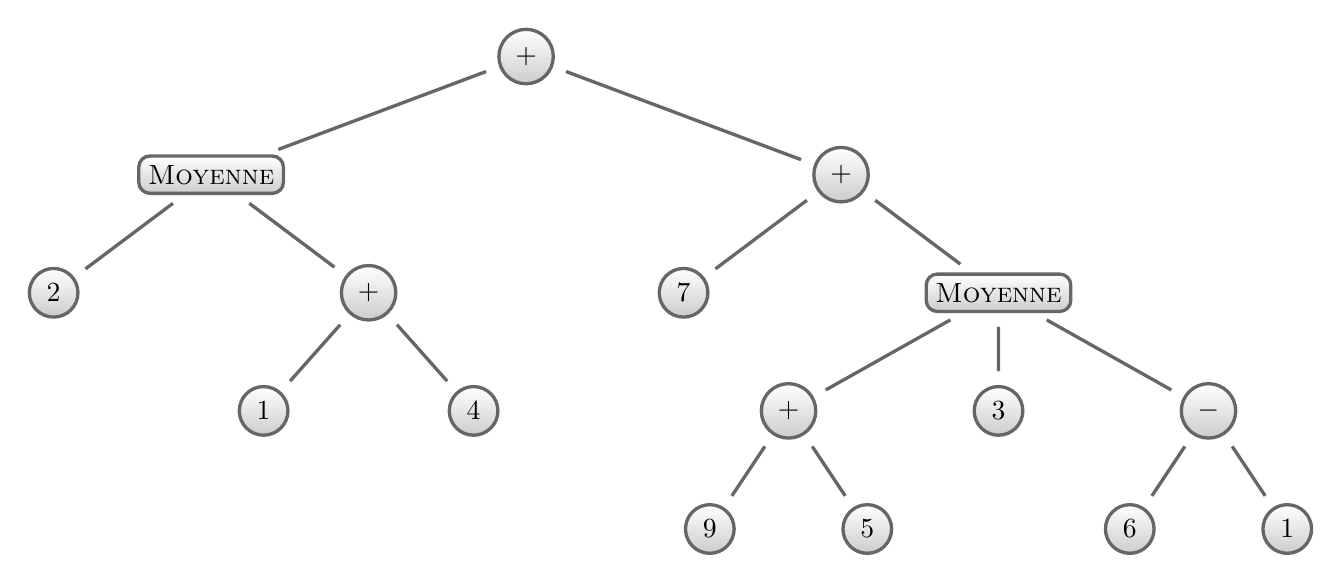
\begin{tikzpicture}[grow=down,level/.style={sibling distance=80mm/#1},punkt/.style={rectangle, rounded corners, shade, top color=white,
    bottom color=black!50!black!20, draw=black!60, very
    thick },edge from parent/.style={very thick,draw=black!60,
	        shorten >=5pt, shorten <=5pt},]

	\node [punkt,circle] (a){$+$}
	  child { node [punkt] (b) {\sc Moyenne}
         child { node [punkt,circle] (c) {$2$} }
         child { node [punkt,circle] (d) {$+$} 
             child { node [punkt,circle] (e) {$1$} }
             child { node [punkt,circle] (f) {$4$} }
               }
	  }
	  child { node [punkt,circle] (g) {$+$}
         child { node [punkt,circle] (h) {$7$} }
         child { node [punkt] (i) {\sc Moyenne}
             child { node [punkt,circle] (j) {$+$} 
                 child { node [punkt,circle] (k) {$9$} }
                 child { node [punkt,circle] (l) {$5$} }
                   }
             child { node [punkt,circle] (m) {$3$} }
             child { node [punkt,circle] (n) {$-$} 
                 child { node [punkt,circle] (o) {$6$} }
                 child { node [punkt,circle] (p) {$1$} }
                   }        
               }
	  }
	 ;

\end{tikzpicture}}
\end{center}

\begin{Question}
  Proposer une hiérarchie de classes permettant de modéliser le
  problème. Identifier les classes qui seront abstraites.
\end{Question}

\begin{Question}
  Dessiner le schéma mémoire de l'objet correspondant à l'expression
  donnée  ci-dessus.
%$$ \textsc{Moyenne}(2, 1 + 4) + (7 + \textsc{Moyenne}(9 + 5, 3, 6 - 1)) $$
\end{Question}

\begin{Question}
  Pour calculer la valeur d'une expression, que doit-on ajouter comme
  primitives (attributs et méthodes) et dans quelles classes ?
  Dessiner le graphe d'héritage avec les attributs et les méthodes
  (uniquement leur profil).
\end{Question}

% \Question Écrire le corps des différentes méthodes nécessaires à
% l'évaluation d'une expression.

On souhaite maintenant étendre nos expressions en autorisant la
définition et l'utilisation de variables. Une même expression pourra
ainsi être réduite en fonction des valeurs de ses variables.  Par
exemple, on définit une variable $x = 3$ et on souhaite évaluer
l'expression $ max(x+2, 7, 9)$.  Il faut donc être capable de lier le
nom de la variable $x$ avec la valeur $3$. Puis, il faut pouvoir
remplacer $x$ par sa valeur dans l'expression. L'expression ci-dessus
se réduit ainsi à la valeur $9$.

\Question Définir une nouvelle classe \texttt{Variable} qui doit
permettre de manipuler des expressions particulières que sont les
variables ainsi que la classe \texttt{Contexte} pouvant contenir
différentes définitions de variables liées.

% \Question Définir une méthode \texttt{calcule(ctx:Contexte):Double}
% pour quelques classes représentatives. Cette méthode remplace toutes
% les occurrences de variables liées par leur valeur avant de calculer
% l'expression. On suppose tout d'abord que toutes les variables sont
% liées dans le contexte.

\Question On souhaite pouvoir réduire une expression dans un contexte
laissant certaines variables libres. La réduction de
$min(x+y, y, x, 9)$ dans le contexte contenant $x=3$ donne
$min(3+y, y, 3)$. On ne peut pas terminer le calcul car $y$ est encore
libre, mais on a remplacé $x$ par sa valeur et déjà calculé le minimum
entre cette valeur et 9. Indiquez le profil des méthodes à définir
dans chaque classe, et donnez l'intuition de leur fonctionnement (sans
forcément écrire de code).

%%%%%%%%%%%%%%%%%%%%%%%%%%%%%%%%%%%%%%%%%%%%%%%%%%%%%%%%%%%%%%%%%%%%%%%%%
%%%%%%%%%%%%%%%%%%%%%%%%%%%%%%%%%%%%%%%%%%%%%%%%%%%%%%%%%%%%%%%%%%%%%%%%%
\bigskip
\Exercice{\bf Questions de synthèse} (8 points).

% L'un des attraits du Scala est de faire le pont entre les langages
% fonctionnels et très fortement typé comme Caml ou Haskell, et des
% langages orientés objets comme Java ou C++. Il est donc intéressant de
% réfléchir à la gestion du typage en Scala en particulier au niveau de
% son interaction avec la manipulation des classes et des objets.

\Question
Présentez comment les notions d'héritage, d'interfaces et de
polymorphisme permettent de factoriser du code au sein d’une
application en vous appuyant sur des exemples. 

\Question Discutez les notions de \emph{co-variance},
\emph{non-variance}, \emph{contra-variance} et
\emph{sous-typage}.
% Étendez votre comparaison au cas des types génériques.

\Question Rappelez le problème classique lié à l’héritage multiple, et
discutez la solution proposée par Scala par rapport à d’autres
langages que vous pouvez connaître.

\Question Quelles notions POO du cours n'étaient pas reprises par les
différentes fourmis à implémenter dans le projet \textit{Ants
  vs. SomeBees}? Quelles créatures pourriez-vous imaginer pour mettre
ces notions à l'œuvre?


% \section{Programmation à objets}

% La seconde partie du cours a été consacrée à l'étude de la
% programmation à objets en appui sur le langage Scala. 
% \begin{description}

% \item [Principes fondamentaux.]  Caractérisez la programmation à
%   objets au travers des différents concepts fondamentaux de cette
%   approche et rappelez pour chaque concept sa syntaxe en
%   Scala. Discutez également l’intérêt et présentez la syntaxe des
%   notions de \emph{paquets}, \emph{modules}, et
%   \emph{exception}. Discutez les interactions entre le mécanisme de
%   polymorphisme et la variance des paramètres.

% \item[Types et classes.]  Comparez les avantages et inconvénients de
%   ces deux notions, en donnant des exemples typiques d’usage. Quand et
%   comment peut-on combiner programmation à objets et programmation
%   fonctionnelle? Quel est le rapport avec la mutabilité des données?

% \item[Composer des types, des objets ou des fonctions.]  Comparez les
%   mécanismes pour déclarer de nouveaux types et ceux de typage
%   automatique d’expressions en Caml et Scala. Discutez des grands
%   principes d’organisation du code et styles de programmation
%   classiques avec des objets ou en fonctionnel.

% \end{description}

\end{document}

  

%%% Local Variables:
%%% mode: latex
%%% TeX-master: t
%%% End:

%  LocalWords:  PROG Luc Quinson mn PC  pt
%  LocalWords:  co-variance non-variance contra-variance
